\subsection{\texorpdfstring{Continuous functions on a compact subset of \(C^{\Lambda}\)}{Continuous functions on a compact subset of C\^{}\{Lambda\}}}

Let \(\Lambda\) be a set and X a compact subset of \(\mathbf{C}^{\Lambda}\) . We denote by P(X) the unital Banach subalgebra of \(\mathcal{C}(\mathrm{X})\) consisting of the functions on X that are uniform limits on X of polynomial functions on \(\mathbf{C}^{\Lambda}\) . The coordinate functions \(z_{\lambda}|\mathrm{X}\) topologically generate P(X), and P(X) separates the points of X. Let Y be the polynomially convex hull of X (def. 4 of I, p.~45). Since

\[
\sup _ {z \in \mathrm{Y}} | p (z) | = \sup _ {z \in \mathrm{X}} | p (z) |
\]

(cf. no. 7 of I, p. 44) for all \(p \in \mathbf{C}[(\mathrm{X}_{\lambda})_{\lambda \in \Lambda}]\) , uniformly convergent sequences of polynomials on X extend uniquely to uniformly convergent sequences of polynomials on Y. There therefore exists a unique isometric isomorphism from P(X) onto P(Y) which, for every coordinate function \(z_{\lambda}\) on \(\mathbf{C}^{\Lambda}\) , maps \(z_{\lambda}|X\) to \(z_{\lambda}|Y\) . This isomorphism will be said to be canonical.

PROPOSITION 4. — Let X be a compact space. Let B be a unital Banach subalgebra of \(\mathcal{C}(\mathrm{X})\) , equipped with the induced norm, separating the points of X. One identifies X with a closed subset of \(\mathrm{X(B)}\) (prop. 1 of I, p.~142, d)). Let \((x_{\lambda})_{\lambda \in \Lambda}\) be a family of elements of B topologically generating the unital algebra B. We consider the commutative diagram

\pandocbounded{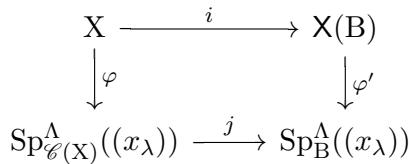
\includegraphics[keepaspectratio]{images/part001_f1662ccb.jpg}}

where \(\varphi\) and \(\varphi'\) are the mappings defined by the family \((x_{\lambda})_{\lambda \in \Lambda}\) (cf. no. 6 of I, p. 41), and \(i\) and \(j\) are the canonical injections. Then:

\begin{enumerate}
\def\labelenumi{\alph{enumi})}
\item
  The maps \(\varphi\) and \(\varphi'\) are homeomorphisms;
\item
  The simultaneous spectrum \(\mathrm{Sp}_{\mathrm{B}}^{\Lambda}((x_{\lambda}))\) is the polynomially convex hull of \(\mathrm{Sp}_{\mathcal{C}(\mathrm{X})}^{\Lambda}((x_{\lambda}))\) ;
\item
  The map \(\varphi\) maps \(\mathcal{C}(\mathrm{X})\) to \(\mathcal{C}(\mathrm{Sp}_{\mathcal{C}(\mathrm{X})}^{\Lambda}((x_{\lambda})))\) and B to \(\mathrm{P}(\mathrm{Sp}_{\mathcal{C}(\mathrm{X})}^{\Lambda}((x_{\lambda})))\) ;
\item
  The map \(\varphi^{\prime}\) maps \(\mathcal{G}_{\mathrm{B}}(\mathrm{B})\) to \(\mathrm{P}(\mathrm{Sp}_{\mathrm{B}}^{\Lambda}((x_{\lambda})))\) ;
\item
  The maps \(\varphi\) and \(\varphi'\) map \(\mathcal{G}_{\mathrm{B}}\) to the canonical isomorphism from \(\mathrm{P}(\mathrm{Sp}_{\mathcal{C}(\mathrm{X})}^{\Lambda}((x_{\lambda})))\) onto \(\mathrm{P}(\mathrm{Sp}_{\mathrm{B}}^{\Lambda}((x_{\lambda})))\) .
\end{enumerate}

The maps \(\varphi\) and \(\varphi'\) are continuous and surjective (I, no. 6, p.~41). The map \(\varphi'\) is a homeomorphism by assertion \(a\) ) of prop. 12 of I, p.~43, and \(i\) is injective, therefore \(\varphi\) is injective. Therefore \(\varphi\) and \(\varphi'\) are homeomorphisms.

Let \(X_{1} = \mathrm{Sp}_{\mathcal{C}(X)}^{\Lambda}((x_{\lambda}))\) . The polynomially convex hull of \(X_{1}\) is \(Y_{1} = \mathrm{Sp}_{\mathrm{B}}^{\Lambda}((x_{\lambda}))\) by prop. 14 of I, p.~46.

For every \(\lambda\in\Lambda\) , let \(z_{\lambda}\) be the corresponding coordinate function on \(\mathbf{C}^{\Lambda}\) . The map \(\varphi\) maps \(x_{\lambda}\) to \(z_{\lambda}|X_{1}\) , and \(\varphi'\) maps \(\mathcal{G}_{\mathrm{B}}(x_{\lambda})\) to \(z_{\lambda}|Y_{1}\) . Therefore \(\varphi\) maps B onto \(\mathrm{P}(X_{1})\) , and \(\varphi'\) maps \(\mathcal{G}_{\mathrm{B}}(B)\) onto \(\mathrm{P}(Y_{1})\) . Finally, \(\varphi\) and \(\varphi'\) map \(\mathcal{G}_{\mathrm{B}}\) to the canonical isomorphism from \(\mathrm{P}(X_{1})\) onto \(\mathrm{P}(Y_{1})\) .

COROLLARY 1. --- Let \(\Lambda\) be a set and X a compact subset of \(\mathbf{C}^{\Lambda}\) . We identify X with a subset of \(\mathsf{X}(\mathrm{P}(\mathrm{X}))\) (prop. 1 of I, p.~142, d)). Let \((z_{\lambda})_{\lambda \in \Lambda}\) be the family of coordinate functions on \(\mathbf{C}^{\Lambda}\) .

\begin{enumerate}
\def\labelenumi{\alph{enumi})}
\item
  The map \(\theta\) from \(\mathrm{X}(\mathrm{P}(\mathrm{X}))\) onto \(\mathrm{Sp}_{\mathrm{P}(\mathrm{X})}^{\Lambda}((z_{\lambda}))\) defined by the family \((z_{\lambda})\) is a homeomorphism from \(\mathrm{X}(\mathrm{P}(\mathrm{X}))\) onto the polynomially convex hull \(Y\) of \(X\). Its restriction to \(X\) is the identity map of \(X\) ;
\item
  For every function \(f \in \mathrm{P}(\mathrm{X})\) , the homeomorphism \(\theta\) transforms the extension \(\mathcal{G}_{\mathrm{P}(\mathrm{X})}(f)\) of \(f\) to \(\mathrm{X}(\mathrm{P}(\mathrm{X}))\) into an extension \(\widetilde{f}\) of \(f\) to \(\mathrm{Y}\) . The map \(f \mapsto \widetilde{f}\) is the canonical isomorphism from \(\mathrm{P}(\mathrm{X})\) onto \(\mathrm{P}(\mathrm{Y})\) .
\end{enumerate}

In prop. 4, take B = P(X) and \(x_{\lambda} = z_{\lambda}\) . Then \(\varphi\) becomes the identity map and \(\varphi'\) becomes the map \(\theta\) . The assertions of the corollary then reduce to those of loc. cit.

COROLLARY 2. --- Let \(\Lambda\) be a set and let \(X \subset \mathbf{C}^{\Lambda}\) be a compact set. If \(X\) is connected, then its polynomially convex hull is connected.

If X is connected, the only idempotents of \(\mathcal{C}(\mathrm{X})\) , hence of \(\mathrm{P}(\mathrm{X})\) , are 0 and 1 (cor. of prop. I, p.~79). Consequently, the space \(\mathrm{X}(\mathrm{P}(\mathrm{X}))\) is connected (loc. cit.); but this set is homeomorphic to the polynomially convex hull of X (cor. 1, a)).

